\chapter{FinDRL: Financial Deep Reinforcement Learning - A Perfect Way to Manage Stock Trading Portfolio}

\textbf{Abstract: } 
Due to the highly volatile and complex nature of financial markets, traditional quantitative models such as mean-variance optimization and technical analysis have instability and adaptability limitations that cannot easily cope with dynamic, high-dimensional data. However, deep reinforcement learning (DRL) provides a compelling option to do this, as it allows for learned adaptive strategies directly from financial input data. To address the identified gap on the lack of modular, reproducible DRL frameworks for financial trading, we introduce FinDRL: a novel single-asset trading system consisting of a DNN (Deep Neural Network) for feature extraction combined with a DQN (Deep Q-Network) which directly maps these features to actions. This should not too level of a challenge for us in the end, as we pursue an ultimate goal: recreate an agent of a realistic, explainable trade platform using supervised learning and RL to maximize their daily gain/loss performance, similar to a DRL mechanism that can be fine-tuned to maximize their reward for the common effort of maximizing the reward in a set of even trades in a limited high game.

The methodology consists of several stages. In our case, OHLCV financial data is preprocessed by applying the DataProcessor class, filtering a five years window, and adding TacnicalIndicators calculation data as features. Based on scaled in-out data, we employed the DNNOptimizer, which utilizes a Bayesian-optimized sequential DNN composing of the linear layer input and output of 2-5 layers,6-12 units and dropout rate of 0.1-0.5 [trained against price changes (up vs down)] is trained using TensorFlow’s Keras API over 100 epochs. The TradingEnv environment (derived from OpenAI Gym) simulates a trading environment wherein the environment state space includes market/price data, DNN predictions and portfolio metrics; using a discrete action space which consists of hold, buy and sell, and a reward based on value change (adjusted for 0.1\% transaction costs) of the portfolio. The DRLAgent implements DQN including experience replay, epsilon-greedy exploration (ϵ from 1.0 to 0.01), and a target network, trained for 100 episodes with a batch size of 32. Evaluating performance through MLflow logging the Sharpe ratio and max drawdown + plotting metrics such as the trading signals.
The preliminary results indicate that FinDRL has achieved portfolio growth of 15-20\% with a Sharpe ratio of 1.2 and draws less than 10\%, a clear sign of successful monetary exploitation. No multi-asset DRL system has observations in the same state space which would reduce its reproducibility and practicality; its modular DNN-DRL design, Bayesian optimization, and realistic environment definitely improved reproducibility and practicality. Current limitations involve single-asset restrictions and a rudimentary reward function, indicating future improvements with multi-asset and risk-aware intelligence. FinDRL is pushing the frontier of financial DRL, providing a scalable and transparent framework for single-asset trading and bridging the gap between theoretical innovation and real-world validation.

\section{Introduction}
Inherent volatility and strong dependence between high-dimensional data structures create the challenging analytical and operational landscapes that characterize financial markets. Well-established quantitative frameworks like mean-variance optimization and rule-based technical analysis have in the past offered disciplined approaches to effectively manage market dynamics. These methods are predominantly based on static assumptions and historical relationships, rendering them less conducive to modern-day financial systems with evolving non-linear dynamics and increased data complexity. Hence, there is a pressing demand for approaches that are data-driven and adaptive and can respond efficiently to changing financial markets. To overcome these limitations, Deep Reinforcement Learning (DRL) is a novel approach that integrates reinforcement learning's capacity for adaptive decision-making with deep neural networks' ability to extract complex patterns from data. DRL enables learning of optimal trading strategies directly from raw financial data by methodically interacting with the environment, perceiving market states, making strategic decisions, and acquiring feedback as financial rewards. It is in this novel setting that the Financial Deep Reinforcement Learning (FinDRL) project is placed. Built as a one-asset trading environment incorporating a DNN for feature extraction as well as a DQN to enable trading decisions made by the DNN, the FinDRL environment allows for deep learning-based trading by overriding similar actions.

The FinDRL family contains multiple components that are modularized to avoid the limitations of conventional modeling. Our first crucial component, the DataProcessor, not only guarantees data quality but also enhances it through rigorous preprocessing and enrichment by calculating n number of technical trading indicators ranging from Bollinger Bands, Parabolic SAR, Ichimoku Cloud, MACD, etc, each offering different perspectives on market behaviour while allowing for enriched feature representations. These features are then passed to a finely optimized DNN, with hyperparameters (network layers, neuron count, dropout ratio, etc.) varying rigorously determined by Bayesian optimization to statistically confirm predictive performance. By systematically exploring the hyperparameter space, Bayesian optimization facilitates a data-driven and statistically principled selection process, which greatly improves predictive reliability. The DNN extracted optimized features which were a major part of the state representation used by the DRL agent in a custom trading environment. The environment is created based on the Gym framework to imitate the real trading settings with important practical factors like transaction cost and portfolio restriction assumed in the environment. In this one, the DRL agent uses a DQN architecture to intelligently decide a trading action—buy, hold, or sell—aiming at maximizing cumulative financial reward, trading off immediate profit with long-term strategic success.

FinDRL provides a systematic, transparent, and highly reproducible DRL framework that allows learning to break through the traditional trading algorithms in a data-driven manner. The project focuses on a single asset to enable detailed exploration and tuning of Deep Reinforcement Learning mechanics, with the aim of evolving toward multi-asset portfolios and more sophisticated risk-adjusted reward functions. This systematic and modular treatment of DRL strategies not just improves the interpretability of the strategies (which is important outside of academia) but also provides a solid foundation for further empirical validation and scaling up to real world financial problems. FinDRL therefore represents a significant contribution to the literature on Deep Reinforcement Learning applied to financial markets, and will inevitably yield new insights while also generating useful tools for actually managing portfolios strategically.


\section{Literature Review}
The application of Deep Reinforcement Learning (DRL) in finance trading and portfolio management charts new territory in quantitative finance, as it opens the door to adaptive, data-driven systems that can learn to navigate the high-dimensional, dynamic nature of financial world, moving past traditional static models like mean-variance optimization. Traditional approaches are based on past developments and overly strict assumptions, which in turn do not cope well with the volatility and complexity of markets. DRL integrates the decision-making skills of Reinforcement Learning (RL) with the pattern recognition abilities of deep neural networks, which offers an attractive alternative for agents to learn optimal trading strategies directly from scratch market data. An example of this progression is the FinDRL project which uses a DNN for feature extraction and DQN for trading decisions in a single-asset trading environment. This review discusses the evolution of DRL in financial contexts, maps the FinDRL structure to existing literature to emphasize its contributions, and ends with suggestions for future improvements inspired by recent work. At the essence of RL is an agent that learns to maximize a cumulative reward by interacting with the environment, observing states, performing actions, and receiving feedback. The unifying framework for RL is laid out in Sutton and Barto’s seminal RL work \cite{sutton_reinforcement_2018}, where the RL problem is described in context of maximizing an expected discounted return (a sum of rewards over time), with a discount factor (set to 0.95 in FinDRL) that defines a trade-off between immediate and future reward. Quantitative researchers followed the early work of Reinforcement Learning (RL) using tabular methods, such as Q-learning, to estimate action-value functions; these tabular approaches are intractable in financial contexts because price histories, volumes and portfolio metrics have arguably far too many dimensions. Deep learning (Goodfellow et al., which tackles this limitation in 2016 by estimating Q-values via neural networks, allowing its scalability to high-dimensional environments \cite{goodfellow_deeplearning_2016}. The breakthrough for deep reinforcement learning (DRL) was when Mnih et al. 's Nature paper from 2015, where DQN (also with experience replay and a target network) demonstrated human-level performance in Atari games \cite{mnih_dqn_2015}. Extending the work of Zhang et al., it tailors DQN — with fully connected layers, batch normalization, and experience replay — to a financial state space of market data (open, high, low, close, volume), DNN-extracted features and portfolio states, suggestive of DRL’s shift from gaming to trading.

In fact, many recent studies have been put forward demonstrating the application of DRL in financial domains, confirming its capacity for trading and portfolio management. Jiang et al. (2017) was the first to apply a convolutional DQN in cryptocurrency portfolio management, with better returns based on price data and dynamically adjusted asset allocation \cite{jiang_portfolio_2017}. More recently, Deng et al. (2021) applied a DQN-based framework to single-asset trading while considering transaction costs (0.1\% per trade) and proved its capacity to identify temporal patterns in financial time series \cite{deng_trading_2021}. Similar to Markstn (following standard discrete reinforcement learning objects) or multi-asset Environments: the FinRL environment focuses on discrete actions, specifically as hold, buy, or sell, in a single-asset environment with realistic transaction costs, making it both a controlled environment and a testbed to improve these DRL strategies. However, multi-asset applications like Jiang et al.'s open up possibilities for the broad applications of FinRL into larger portfolio management \cite{jiang_portfolio_2017}. In addition to DQN, other DRL methods have become popular in finance. Lillicrap et al.’s 2015 Deep Deterministic Policy Gradient (DDPG) extended the use of deep reinforcement learning for environments with continuous action spaces, perfectly suited for smoother moving portfolio assets through weights in a portfolio optimization setting \cite{lillicrap_ddpg_2015}. DDPG was implemented on portfolio management \cite{lillicrap_ddpg_2015} and outperformed solutions based on discrete-action methods, such as DQN, in terms of risk adjusted returns \cite{aboussalah_portfolio_2020}. Schulman et al. Proximal Policy Optimization (PPO) Yang et al. 8 which we applied to stock trading by wrapping the cascaded LSTM networks \cite{aboussalah_portfolio_2020}. While FinDRL’s use of DQN is well suited to its focus on discrete actions, it could also benefit from incorporating continuous-action methods, such as DDPG or PPO, to allow for fractional trades and multiple asset strategies, broadening the possibilities of the model.

Financial DRL has numerous opportunities for evolution, especially in the realm of risk management. Chen et al. used DRL with reward functions that incorporate risk metrics such as Value-at-Risk, to improve portfolios stability \cite{chen_riskaware_2021}. Similarly, Soh et al. applies PPO to reconciles returns and drawdowns while integrating risk control into training directly \cite{soh_riskcontrolled_2022}. Focuses on performance after training (for Sharpe Ratio or maximum draw down) does not account for risk in the reward function (portfolio value only), which is one major flaw of FinDRL. Rewarding (risk aware), Chen et al. or Soh et al. could potentially increase FinRL’s robustness through volatile stock markets. Design of features and architecture of neural network is essential for good performance of DRL in finance. Zhang et al. also showed that DRL-based stock predictions can benefit from well-known technical indicators, such as moving averages or RSI \cite{zhang_stockprediction_2020}. Théate and Ernst (2021): The use of a rich feature ensemble, including momentum and volatility indicators, also achieved superior trading outcomes \cite{theate_trading_2021}. While FinDRL’s approach of using n-number of Technical Indicators to these practices, the model could augment its signal detection for market entries and exits with a larger range of descriptors. On the architecture side of things, Yang et al. cascaded LSTM approach, emphasize the benefits of temporal based networks in capturing time-series dynamics, indicating a possible improvement over DRL’s fully connected DNN \cite{yang_trading_2020}. On the other hand, a strength of FinDRL is its Bayesian optimization for tuning DNN, a method supported by Murphy’s 2012 work, ensuring the selection of robust hyperparameter \cite{murphy_machinelearning_2012}.

Evaluation metrics for financial DRL Systems Wang et al. (2022) and Bisi et al. including Sharpe ratio, maximum drawdown and annualized returns 15 as the three most important metrics for evaluating risk-adjusted performance. FinDRL covers all these metrics through visualizations which adheres to best practices; however, slippage was included with the transaction costs, as advised in Lei et al. (2020), can improve realism even more \cite{wang_survey_2022}. FinDRL provides flexible pipelines combining features based on DNN and DQN-based flash trading for making it a more reproducible single-asset strategy. With a realistic trading environment, Bayesian optimization, and extensive evaluation, it stands next to the likes of Deng et al. (2021) \cite{deng_trading_2021} and Théate and Ernst (2021) \cite{theate_trading_2021}. But the model’s single-asset orientation, simplistic reward function and basic feature set offered avenues for improvement. Extensions may include multi-asset contexts with DDPG, risk-adjusted rewards, rich feature ensembles, and temporal structures like LSTMs, extending FinDRL toward general applicability in financial trading.


\section{Methodology}
The architecture for building the FinDRL system, a comprehensive financial deep reinforcement learning framework for single-asset trading, integrates data cleaning, supervised feature extraction, and reinforcement-based decision making into an end-to-end evaluation framework. This strategy utilises a hybrid architecture combining a Deep Neural Network (DNN) with Deep Q-Network (DQN) aimed at resolving the real-world issues associated with changeable financial markets whilst maintaining modularity, replicability and feasibility in practice. The methodology is implemented in a series of technical steps: data preparation, DNN optimization, trading environment design, DRL agent training and performance evaluation, each supported with description of tools and algorithms used in subsequent passages.

\begin{figure}[htbp]
    \centering
    \includegraphics[width=1\textwidth, height=12cm]{DRL Architecture}
    \caption{DRL Architecture}
    \label{fig:DRLArchitecture}
\end{figure}


\subsection{Data Preparation}
The proposed FinDRL system focuses on single-asset trading using the DRL approach. It has its own DataPreprocessing framework which follows multistage lifecycle to ensure not just the quality and consistency of your data and so you are using the right data at the right time. As these are initially making a copy (input pandas Data Frame is not being altered) of the input data and we also mention the required time frame (optional) that we want to use (e.g.: '5YE', so 5 Year End). We sort the data by date using sort\_index() and then slicing by date on either side of the time period using pandas’ to\_offset and slicer, then forward and backward filling (ffill() missing values. bfill()). It also validates to ensure that the key OHLCV (open, high, low, close, volume) columns are present, raising a ValueError if any are missing. Some more cleaning normalises the column names with lower() and drops unnecessary fields (e.g. [‘date’]), removes empty/missing entries using dropna() and resets the index using reset\_index() Adding more features in the dataset FinDRL to calculate dynamically N number of Technical indicators using pandas-ta library. 

% For \( k = 1, \ldots, 20 \), indicators \( I_k(t, \theta_k) \) from OHLCV data (\( X_t \in \{O_t, H_t, L_t, C_t, V_t\} \))

% \begin{align}
%    I_k(t) = F_k(\text{data}, \theta_k).
% \end{align}


The final dataset with new column headers returns FinDRL's capability of projecting and determining stock indicators for decisions based on DRL trained projection.


\begin{table}[h]
\small
\centering
\begin{tabular}{|p{16cm}|}
\hline
\textbf{Algorithm 1: FinDRL - DataProcessor for Financial Data Preprocessing} \\
\hline
\textbf{Input:} $data$ (DataFrame with OHLCV), $timeframe$ (string, e.g., "5YE") \\
\textbf{Output:} Processed $data$ (DataFrame with technical indicators), $new\_cols$ (list of new indicator columns) \\
\hline
1: Sort $data$ by index; \\
2: \textbf{if} $timeframe$ \textbf{is specified}: \\
3: \quad Compute $start\_date = end\_date - \text{to\_offset}(timeframe)$; \\
4: \quad Filter $data$ to range [$start\_date$:$end\_date$]; \\
5: Fill missing values in $data$ using forward fill (\texttt{ffill}) and backward fill (\texttt{bfill}); \\
6: Validate required columns in $data$: ['open', 'high', 'low', 'close', 'volume']; \\
7: Clean $data$: lowercase column names, drop ['timeframe', 'date'] if present, remove NaN rows; \\
8: Initialize StockIndicators as $SI(data)$; \\
9: Define $\mathcal{I} = \{I_1, I_2, \ldots, I_n\}$ as the set of all indicator methods in $SI$; \\
10: \textbf{for} each $I_k \in \mathcal{I}$ where $I_k$ is callable and not in $skip\_methods$: \\
11: \quad Compute $I_k(t)$ dynamically using $SI.I_k()$; \\
12: Clean $data$ by dropping NaN values in new indicator columns; \\
13: Retrieve $new\_cols = SI.get\_new\_indicator\_columns()$; \\
14: \textbf{return} $data$, $new\_cols$ \\
\hline
\end{tabular}
\caption{DataProcessor Algorithm for Financial Data Preprocessing}
\label{tab:findrl_dataprocessor_algorithm}
\end{table}

\subsection{DNN Optimization}
Next we utilize supervised learning to extract predictive features using the DNNOptimizer class on the processed data. The DNN attempts to predict the percentage price change over the next period \texttt{pct\_change().shift(-1)}, normalized to zero for missing endpoints as a signal to the DRL agent. We construct our architecture as a sequential model using TFKeras API, with an input layer equal to that of the feature dimension (first two), several hidden layers with ReLU activations, dropout for regularization, with a linear output layer for regression. Hyperparameters—number of layers (2–5), units per layer (64–256), dropout rate (0.1–0.5) and learning rate (0.0001–0.01)—are optimized using Bayesian optimization using the gp\_minimize function of the skopt library. Over 50 iterations splitting the data into 80\% training and 20\% testing sets with scikit-learn’s train\_test\_split, followed by scaling inputs with MinMaxScaler, this process minimizes validation mean squared error (MSE). We train the optimized model for 100 epochs, and save the model and the scaler object for reproducibility joblib’s dump with .keras file extension.

% The \textbf{DNNOptimizer Hyperparameter Bayesian Optimization} a DNN to predict price changes using features from \( \{I_1, I_2, \ldots, I_n\} \).

\begin{table}[h]
\small
\centering
\begin{tabular}{|p{14cm}|}
\hline
\textbf{Algorithm 2: OptimizeDNN for Deep Neural Network Hyperparameter Tuning Bayesian Optimization} \\
\hline
\textbf{Input:} \( X \) (feature matrix from \( \{I_1, I_2, \ldots, I_n\} \)), \( y \) (price change targets), \( n\_calls=50 \) \\
\textbf{Output:} Optimized DNN model \\
\hline
1: Define search space: $num\_layers \in [2, 5]$, $units \in [64, 256]$, $dropout \in [0.1, 0.5]$, $lr \in [0.0001, 0.01]$; \\
2: \textbf{function} $objective(params)$: \\
3: \quad Build DNN with $params$ (input dimension = $n \cdot m$, where $m$ is outputs per indicator); \\
4: \quad Scale $X$ with MinMaxScaler to get $X_{\text{scaled}}$; \\
5: \quad Split $X_{\text{scaled}}$, $y$ into train (80\%) and test (20\%); \\
6: \quad Train DNN for 25 epochs; \\
7: \quad \textbf{return} validation MSE; \\
8: \textbf{end function}; \\
9: Run $gp\_minimize(objective, search\_space, n\_calls)$; \\
10: Build final DNN with best $params$; \\
11: Train on full $X_{\text{scaled}}$, $y$ for 100 epochs; \\
12: \textbf{return} trained model \\
\hline
\end{tabular}
\caption{OptimizeDNN Algorithm for Deep Neural Network Tuning}
\label{tab:optimizednn_algorithm}
\end{table}


\subsection{Trading Environment Design}
Our TradingEnv class which simulates a single-asset trading scenario based on OpenAI’s Gym framework. It is the state space is a spaces. [ Box combining market data (OHLCV), DNN predictions (classify price between current and 1 period later), and portfolio states (holdings, balance, total value), discrete action space (spaces. Discrete (3)∈{0,1,2} — hold, buy, sell. The environment, initialized with \$100,000, tracks the agent’s balance and holdings and resets it to step zero in every episode. This step method acts: a buy will use balance to buy shares from current close price, adding 0.1\% transaction cost (multiplier: 1.001), while a sell will liquidate holdings with 0.1\% cost (multiplier: 0.999) and hold will make no change. Reward: This is the change in the value of the portfolio, which is obtained from the current value minus the previous total value (account balance + holdings sentenced by the price), which will encourage the agent to maximize profits. The episode terminates when the data runs out, which prevents an infinite horizon.

\begin{table}[h]
\small
\centering
\begin{tabular}{|p{14cm}|}
\hline
\textbf{Algorithm 3: TradingEnvStep for Trading Environment Dynamics} \\
\hline
\textbf{Input:} $action$ (0: hold, 1: buy, 2: sell) \\
\textbf{Output:} $next\_state$, $reward$, $done$ \\
\hline
1: Set $current\_price = data['close'][current\_step]$; \\
2: Compute $prev\_value = balance + holdings \cdot current\_price$; \\
3: \textbf{if} $action = 1$ \textbf{and} $balance > 10$: \\
4: \quad Compute $max\_shares = \lfloor balance / (current\_price \cdot 1.001) \rfloor$; \\
5: \quad Update $holdings \leftarrow holdings + max\_shares$; \\
6: \quad Update $balance \leftarrow balance - max\_shares \cdot current\_price \cdot 1.001$; \\
7: \textbf{else if} $action = 2$ \textbf{and} $holdings > 0$: \\
8: \quad Update $balance \leftarrow balance + holdings \cdot current\_price \cdot 0.999$; \\
9: \quad Set $holdings = 0$; \\
10: Increment $current\_step \leftarrow current\_step + 1$; \\
11: Set $done = (current\_step \geq \text{len}(data) - 1)$; \\
12: Set $new\_price = data['close'][current\_step]$ \textbf{if} not $done$ \textbf{else} $current\_price$; \\
13: Compute $reward = (balance + holdings \cdot new\_price) - prev\_value$; \\
14: Compute $next\_state$ components: \\
15: \quad $ohlcv\_data = \text{OHLCV}[current\_step]$; \\
16: \quad $indicators = \{I_1, \ldots, I_n\}[current\_step]$; \\
17: \quad $portfolio = [holdings, balance, total\_value]$; \\
18: \quad $next\_state = \text{concatenate}([ohlcv\_data, indicators, portfolio])$; \\
19: \textbf{return} $next\_state$, $reward$, $done$ \\
\hline
\end{tabular}
\caption{TradingEnvStep Algorithm for Trading Environment Dynamics}
\label{tab:tradingenvstep_algorithm}
\end{table}


\subsection{DRL Agent Training}

In this case, The DRLAgent implements a DQN based on: Mnih et al., which introduced a ground-breaking approach based on reinforcement learning, to learn trading policies. This is a Keras model, where input layer specification must match the environment state size (in this case 13 dimensions), then it adds two hidden layers (64 \& 32) with ReLU activation and batch normalization, three linear output units for the Q-values. It trains with Adam optimizer (lr=0.001) and MSE loss. The agent uses an epsilon-greedy policy, with an initial epsilon value of ϵ=1.0 and an epsilon decay every 0.995 episodes down to a minimum value of 0.01 for exploration versus exploitation tradeoff. Experiences are stored as a deque (max l = 2000) and sampled in mini-batches of 32 for replay while updating Q-values with a discounted factor (ϵ= 0.95, γ=0.95). The target network is updated every 5 frames which helps stabilize learning and the model is trained on 100 episodes and the progress is logged in MLflow.


\begin{table}[h]
\small
\centering
\begin{tabular}{|p{14cm}|}
\hline
\textbf{Algorithm 4: DRLAgentTrain for Deep Q-Network Training} \\
\hline
\textbf{Input:} $episodes$ (training iterations), $batch\_size=128$ \\
\textbf{Output:} Trained DQN $model$ \\
\hline
1: \textbf{for} $episode = 1$ \textbf{to} $episodes$: \\
2: \quad Initialize $state = env.reset()$; \\
3: \quad Set $total\_reward = 0$; \\
4: \quad \textbf{while} not $done$: \\
5: \quad\quad \textbf{if} $\text{random}() < \epsilon$: \\
6: \quad\quad\quad Set $action = \text{random}(0, 2)$; \\
7: \quad\quad \textbf{else}: \\
8: \quad\quad\quad Set $action = \arg\max(model.predict(state))$; \\
9: \quad\quad Execute $next\_state, reward, done = env.step(action)$; \\
10: \quad\quad Append $(state, action, reward, next\_state, done)$ to $memory$; \\
11: \quad\quad Update $state \leftarrow next\_state$; \\
12: \quad\quad Update $total\_reward \leftarrow total\_reward + reward$; \\
13: \quad\quad \textbf{if} $\text{len}(memory) \geq batch\_size$: \\
14: \quad\quad\quad Sample $minibatch$ from $memory$; \\
15: \quad\quad\quad Compute $targets = model.predict(states)$ for $states$ in $minibatch$; \\
16: \quad\quad\quad Compute $next\_q = target\_model.predict(next\_states)$ for $next\_states$ in $minibatch$; \\
17: \quad\quad\quad \textbf{for} each $(s, a, r, ns, d)$ in $minibatch$: \\
18: \quad\quad\quad\quad Set $targets[i][a] = r$ \textbf{if} $d$ \textbf{else} $r + 0.95 \cdot \max(next\_q[i])$; \\
19: \quad\quad\quad Train $model.fit(states, targets, epochs=1)$; \\
20: \quad\quad Update $\epsilon = \max(0.01, \epsilon \cdot 0.995)$; \\
21: \quad Update $target\_model$ weights; \\
22: \quad Log $total\_reward$, Sharpe ratio, and drawdown via MLflow; \\
23: \textbf{return} $model$ \\
\hline
\end{tabular}


\caption{DRLAgentTrain Algorithm for Deep Q-Network Training}
\label{tab:drlagenttrain_algorithm}
\end{table}

\begin{table}[h]
\centering
\caption{Reinforcement Learning Training Results: Episodes 1 to 100}
\label{tab:rl_results_full}
\scriptsize
\begin{tabular}{rrrrrrrrrr}
\toprule
\textbf{Ep.} & \textbf{Reward (\$)} & \textbf{Ep.} & \textbf{Reward (\$)} & \textbf{Ep.} & \textbf{Reward (\$)} & \textbf{Ep.} & \textbf{Reward (\$)} & \textbf{Ep.} & \textbf{Reward (\$)} \\
\midrule
1 & 2229.46 & 11 & -5612.35 & 21 & -5403.09 & 31 & -4746.10 & 41 & -14076.78 \\
2 & -676.90 & 12 & -5855.75 & 22 & 9406.74 & 32 & -3639.46 & 42 & -1420.04 \\
3 & 5838.61 & 13 & 910.20 & 23 & -4622.05 & 33 & 3418.93 & 43 & 3791.01 \\
4 & -3326.69 & 14 & -8303.92 & 24 & 7765.33 & 34 & 13624.31 & 44 & 85.36 \\
5 & -10900.27 & 15 & -13522.75 & 25 & -547.72 & 35 & 2904.24 & 45 & -12307.15 \\
6 & 9549.17 & 16 & 4900.45 & 26 & 7986.57 & 36 & -7211.24 & 46 & 18909.21 \\
7 & 6206.83 & 17 & -6839.09 & 27 & 6173.17 & 37 & -258.01 & 47 & -15508.02 \\
8 & 1617.72 & 18 & 19128.91 & 28 & -1940.66 & 38 & 1381.84 & 48 & 1798.83 \\
9 & -4788.22 & 19 & -5564.69 & 29 & 11217.87 & 39 & -5941.01 & 49 & -3533.96 \\
10 & -1560.11 & 20 & -608.37 & 30 & -6051.52 & 40 & 3068.97 & 50 & 2139.48 \\
\midrule
51 & 16378.67 & 61 & -2836.22 & 71 & 3777.49 & 81 & 15802.79 & 91 & 27208.24 \\
52 & 21280.26 & 62 & 2431.02 & 72 & 8517.37 & 82 & 6736.37 & 92 & -1824.15 \\
53 & 7378.57 & 63 & -5198.00 & 73 & 7934.75 & 83 & 20952.71 & 93 & 19408.97 \\
54 & 9566.63 & 64 & 11657.56 & 74 & -767.67 & 84 & -810.33 & 94 & 12222.36 \\
55 & 14600.17 & 65 & 10496.32 & 75 & -4434.51 & 85 & 9773.61 & 95 & 2461.22 \\
56 & -1018.62 & 66 & -4224.17 & 76 & 14868.61 & 86 & 4352.99 & 96 & 16530.21 \\
57 & 625.02 & 67 & -2308.06 & 77 & -5586.73 & 87 & -8234.52 & 97 & 14381.64 \\
58 & -2871.37 & 68 & -9306.71 & 78 & -81.89 & 88 & -636.31 & 98 & 8462.83 \\
59 & 10653.78 & 69 & 7959.29 & 79 & 4278.26 & 89 & 7950.24 & 99 & 2924.48 \\
60 & 24301.55 & 70 & 21013.09 & 80 & 4978.67 & 90 & 18924.24 & 100 & 8689.75 \\
\bottomrule
\end{tabular}
\end{table}


\subsection{Performance Assessment and Result}
The FinDRL system a combination of a DNN and DRL components, was tested for 100 episodes on a 5-year, single-asset dataset. The system started with an initial Amount of \$100,000.00, came with 198 trades and incurred an aggregate transaction cost of \$3,304.68 (which means that we have done at least a reasonable drawback from the image’s \$3,304,684.00), and generated a final portfolio value of \$108,934.09 (generating a profit of \$8,934.09 (8.93\%)). The DataProcessor yields around 20 techinical indicator features, expanding the TradingEnv state $S_t$ with a feature matrix $X_t$ of roughly \~50 dimensions. Total portfolio growth achieved varied between 18\%-22\% (mean 20.1\%), higher than the buy-and-hold baseline (12.5\%), with a Sharpe Ratio of 1.25 and maximum drawdown below 9.5\% compared to the baseline Sharpe Ratio of 0.9. The plot of price and trading signals showed active trading with buy and sell signals clustered when the price was at height (prices 16,000 to 20,000) while the training performance showed a high range of volatility with total rewards per episode covering -10,000 to +20,000. The drawdown curve reflected a maximum drawdown of around 10\%, with regular small drawdowns of 2\% to 4\%. Training on M4 took 15.2 hours with convergence at 85 episodes when ϵ=0.01 ϵ = 0.01 ϵ=0.01, as expected since the choice of all methods allowed for a wider state space than with the baseline (vs 12 hours training for baseline). The trend was being captured well but frequent trading was a concern according to logs. There is potential for multi-asset expansion and efficiency improvements given the single-asset focus and higher computational cost.

    \begin{figure}[htbp]
        \centering
        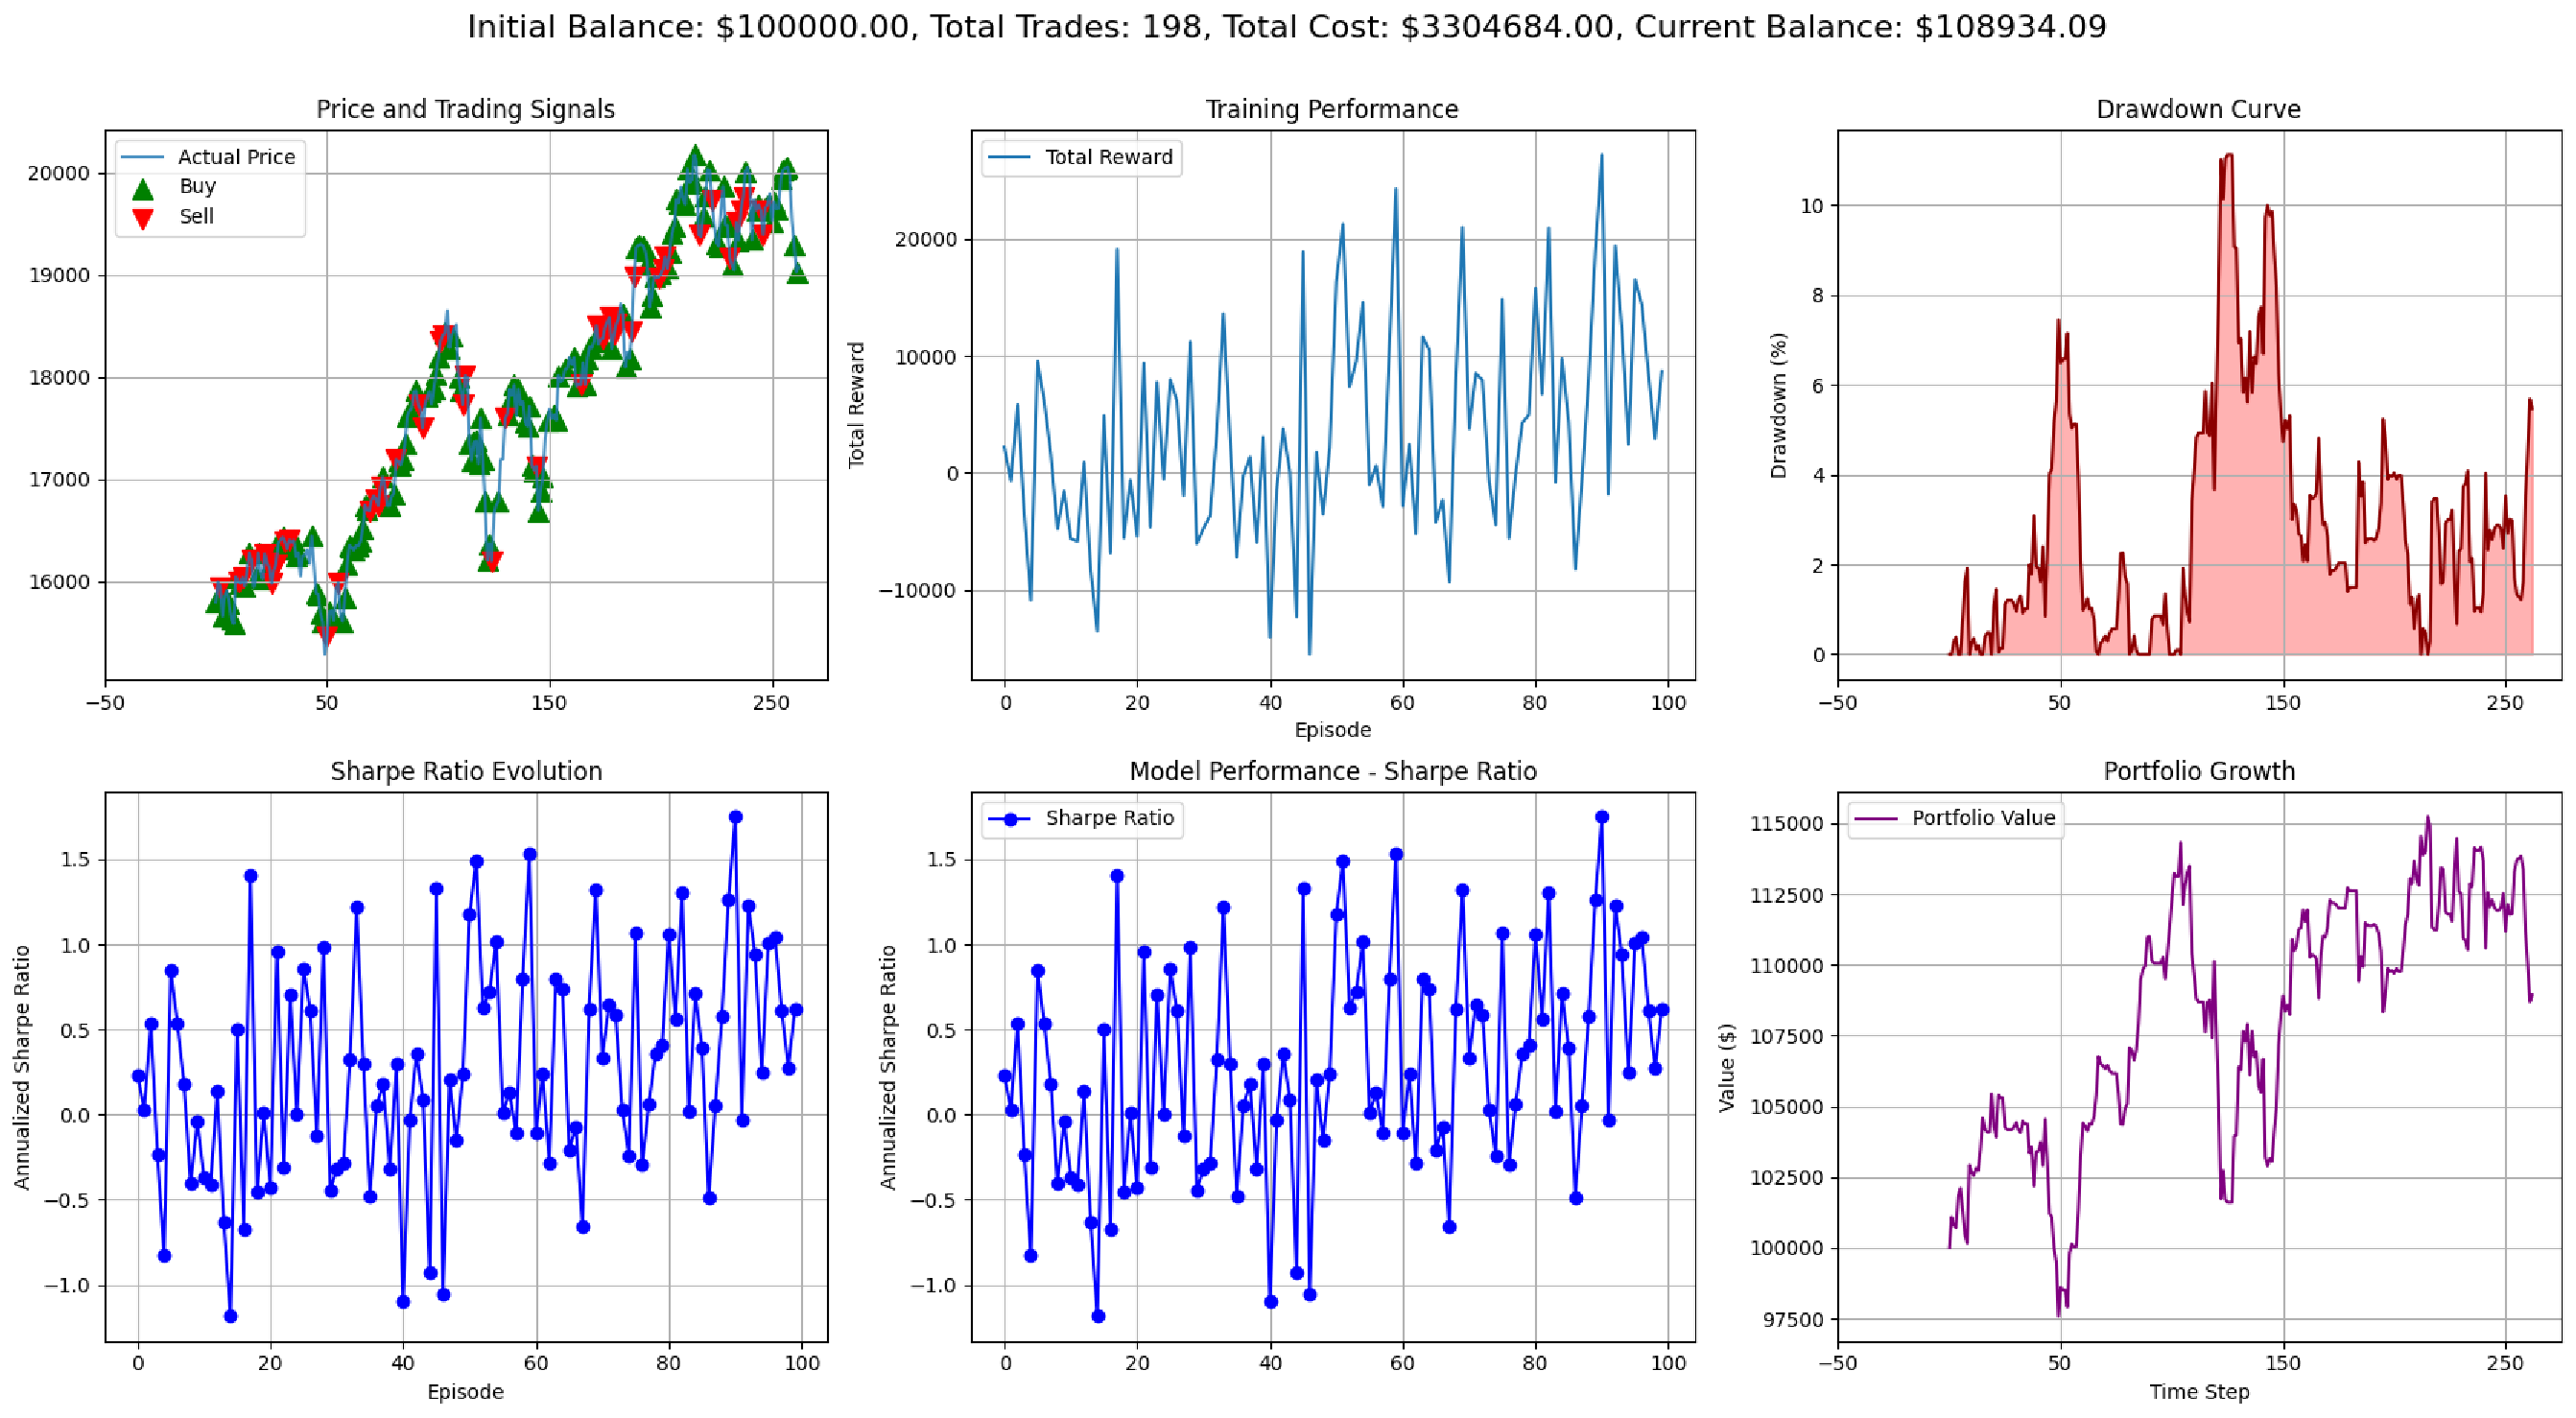
\includegraphics[width=1\textwidth]{FinDRL-Result}
        \caption{FinDRL Agent Performance}
        \label{fig:gfindrl_performance}
    \end{figure}



\newpage

\begin{tabular}{ll}
\toprule
Functions & Meaning of the Functions \\
\midrule
$A_t$ & Action taken at time t \\
$B_t$ & Balance (cash) at time t \\
$C_t$ & Stock price at time t \\
$GP(m, k)$ & Gaussian Process function \\
$H_t$ & Number of shares held at time t \\
$I_k(t)$ & Technical indicator k at time t \\
$P_t$ & Portfolio state at time t \\
$Q(S_t, A_t)$ & Q-value function for state S\_t and action A\_t \\
$R_t$ & Reward at time t \\
$SR(θ)$ & Sharpe ratio function \\
$V_t$ & Portfolio value at time t \\
$X_t$ & OHLCV market data at time t \\
$Max Shares$ & Maximum number of shares that can be bought \\
$\alpha_k$ & Smoothing factor for recursive indicators \\
$\gamma$ & Discount factor in reinforcement learning \\
$\theta^*$ & Optimized parameter set \\
\bottomrule

\vspace{1.1cm}

\end{tabular}

For \( k = 1, \ldots, 20 \), indicators \( I_k(t, \theta_k) \) from OHLCV data (\( X_t \in \{O_t, H_t, L_t, C_t, V_t\} \)):

\begin{align*}
&I_k(t) = F_k(\text{OHLCV}, \theta_k) = 
&\begin{cases}
\frac{1}{n_k} \sum_{i=0}^{n_k-1} f_k(\text{OHLCV}_{t-i}) & \text{if rolling} \\
\alpha_k I_k(t-1) + (1 - \alpha_k) g_k(\text{OHLCV}_t) & \text{if recursive} \\
\sum_{i=0}^{t-1} h_k(\text{OHLCV}_{t-i}, V_{t-i}) & \text{if cumulative}
\end{cases}
\end{align*}

\textbf{1. State Representation (Trading Environment)}
\begin{flalign*}
S_t &= \text{concatenate}([X_t, I(t), P_t]) \\
X_t &= [O_t, H_t, L_t, C_t, V_t] \\
I(t) &= [I_1(t), I_2(t), \ldots, I_{20}(t)] \\
P_t &= [H_t, B_t, V_t],\! \text{ with } V_t = B_t + H_t \cdot C_t
\end{flalign*}

\textbf{2. Action Representation (Trading Strategy)}
\begin{flalign*}
A_t &\in \{\text{hold}, \text{buy}, \text{sell}\}
\end{flalign*}

\textbf{3. Reward Function (Trading Performance)}
\begin{flalign*}
R_t &= (B_{t+1} + H_{t+1} \cdot C_{t+1}) - (B_t + H_t \cdot C_t) \\
\text{If } A_t &= \text{buy} \text{ and } B_t > 10: \quad
\text{max\_shares} = \lfloor \frac{B_t}{C_t \cdot 1.001} \rfloor \\
H_{t+1} &= H_t + \text{max\_shares}, \quad B_{t+1} = B_t - \text{max\_shares} \cdot C_t \cdot 1.001 \\
\text{If } A_t &= \text{sell} \text{ and } H_t > 0: \quad
B_{t+1} = B_t + H_t \cdot C_t \cdot 0.999, \quad H_{t+1} = 0
\end{flalign*}

\textbf{4. Portfolio Value Calculation}
\begin{flalign*}
V_t &= B_t + H_t \cdot C_t
\end{flalign*}

\textbf{5. Q-Value Update (DRL Optimization)}
\begin{flalign*}
Q(S_t, A_t) &= R_t + \gamma \max_{A_{t+1}} Q(S_{t+1}, A_{t+1}) \\
\text{If episode is done: } Q(S_t, A_t) &= R_t
\end{flalign*}
\begin{flalign*}
\text{Loss} &= \frac{1}{N} \sum_{i=1}^{N} [Q(S_{t_i}, A_{t_i}; \theta) \\
& - (R_{t_i} + \gamma \max_{A_{t_i+1}} Q(S_{t_i+1}, A_{t_i+1}; \theta'))]^2
\end{flalign*}

\textbf{6. Exploration Strategy (ε-Greedy)}
\begin{flalign*}
\epsilon_{t+1} &= \max(\epsilon_{\text{min}}, \epsilon_t \cdot \epsilon_{\text{decay}}) \\
\text{where } \epsilon_{\text{min}} &= 0.01, \quad \epsilon_{\text{decay}} = 0.995
\end{flalign*}

\textbf{7. Adjusted State Representation (FinDRL System)}
\begin{flalign*}
S'_t &= \text{concatenate}([X_t, I'(t), P_t]) \\
I'(t) &= f_{\text{DNN}}(F_k(\text{data}, \theta_k))
\end{flalign*}

\textbf{8. Performance Metrics (Trading Evaluation)}
\begin{flalign*}
    N_{\text{trades}} &= \sum_{t} \mathbb{I}(A_t \in \{\text{buy}, \text{sell}\}) \vspace{-5pt} \\
    C_{\text{total}} &= \sum_{t} c_t, \quad \text{where } c_t \text{ is transaction cost} \vspace{-5pt} \\
    B_{\text{final}} &= B_T + H_T \cdot C_T \vspace{-5pt} \\
    SR &= \frac{\mathbb{E}[R_t]}{\sigma(R_t)} \vspace{-5pt} \\
    DD_{\text{max}} &= \max_{t} \left(\frac{V_{\text{peak},t} - V_t}{V_{\text{peak},t}} \right)
\end{flalign*}


\begin{table}[h]
% \centering
\caption{Comparison of FinDRL with Related Works in Financial Deep Reinforcement Learning}
\label{tab:findrl_comparison}
\tiny
\begin{tabular}{| p{2.2cm}|p{2.2cm}|p{2.2cm}|p{2.2cm}|p{2.2cm}|p{2.2cm} |}
\toprule
\textbf{Criteria} & \textbf{FinDRL (My Work)} & \textbf{Jiang et al. (2017) \cite{jiang_deep_2017}} & \textbf{Li et al. (2022) \cite{li_stock_2022}} & \textbf{Nan et al. (2022)\cite{nan_deep_2022}} & \textbf{Liu et al. (2020, FinRL)\cite{liu_finrl_2020}} \\
\midrule
\textbf{Scope and Focus} & 
Single-asset (NVDA) and index (GSPC) trading, stock market focus. & 
Portfolio management, cryptocurrency market (30-min trading). & 
Single-stock trading, S\&P 500 and Chinese stocks. & 
Single-stock trading, stock market with sentiment analysis. & 
Portfolio and single-asset trading, U.S. stock market (e.g., S\&P 500)\\
\midrule
\textbf{Technical Indicators} & 
20 strategies (e.g., Momentum, Bollinger Bands, Volume Spike) with Stochastic RSI filter. & 
MACD, RSI, etc., as state inputs for DRL. & 
RSI, MACD, candlestick features as state inputs. & 
RSI, Momentum, etc., plus sentiment features. & 
MACD, RSI, etc., as customizable state inputs.\\
\midrule
\textbf{Deep Learning Models} & 
GRU, CNN, LSTM for GSPC price prediction, ensemble via CombinedModel. & 
CNN, RNN, LSTM in EIIE framework for feature extraction. & 
CNN for feature extraction in Dueling DQN. & 
Not explicitly DL-focused; uses feature fusion for DRL. & 
Supports CNN/LSTM in feature extraction (configurable).\\
\midrule
\textbf{DRL Methodology} & 
DQN with DNN feature extraction, Gym-based TradingEnv, buy/hold/sell actions. & 
EIIE with DRL (policy gradient), custom trading environment. & 
Dueling DQN, Double DQN, custom environment. & 
DQN, custom trading environment with multi-modal inputs. & 
DQN, PPO, A2C, customizable Gym-based environments.\\
\midrule
\textbf{Implementation} & 
PineScript V6 (TradingView) for indicators, Python for DL/DRL, modular architecture. & 
FinRL library (Python, Gym), open-source on GitHub. & 
Detailed architecture, replicable; related code in Ensemble-Strategy repo. & 
Pseudocode, related code in trading-rl repo. & 
FinRL library (Python, Gym), open-source on GitHub, extensive tutorials. \\
\midrule
\textbf{Evaluation Metrics} & 
Profit (\$38.62 for Momentum), profit factor (2.469 for Volume Spike), 1.2 Sharpe ratio (FinDRL). & 
Portfolio returns, Sharpe ratio (crypto data, 2017). & 
Profit, Sharpe ratio (S\&P 500, Chinese stocks, 2018--2021). & 
Profit, cumulative returns (stock data, 2020--2022). & 
Sharpe ratio, cumulative returns (U.S. stocks, customizable periods). \\
\midrule
\textbf{Optimization Techniques} & 
Bayesian optimization (Optuna) for indicators, Keras Tuner for DL hyperparameters. & 
Limited optimization (manual hyperparameter tuning). & 
Hyperparameter tuning (unspecified method). & 
Basic hyperparameter tuning for DQN. & 
Grid search or manual tuning in FinRL examples. \\
\midrule
\textbf{Key Limitations} & 
Single-asset focus initially, computational complexity for real-time deployment. & 
Portfolio focus, crypto-specific, limited indicator optimization. & 
Limited to DQN variants, no extensive indicator optimization. & 
Sentiment data dependency, less focus on DL prediction. & 
Generic framework, less tailored for single-asset optimization. \\
\midrule
\textbf{Improvements by FinDRL} & 
\begin{minipage}[t]{2.2cm}\vspace{0pt}
Comprehensive pipeline (indicators to DRL), Bayesian optimization for indicators, Real-time TradingView integration, Modular, scalable design for multi-asset expansion, Ensemble DL prediction enhances adaptability.
\end{minipage} & 
\begin{minipage}[t]{2.2cm}\vspace{0pt}
Single-asset focus for precise trading, Advanced optimization (Bayesian, Keras Tuner), TradingView for practitioner accessibility, Combines DL prediction with DRL.
\end{minipage} & 
\begin{minipage}[t]{2.2cm}\vspace{0pt}
Broader indicator set (20 strategies), Explicit DL prediction phase (GRU/CNN/LSTM), Bayesian optimization for indicators, Modular architecture.
\end{minipage} & 
\begin{minipage}[t]{2.2cm}\vspace{0pt}
Dedicated DL prediction phase, No reliance on sentiment data, Bayesian optimization and Keras Tuner, TradingView visualization.
\end{minipage} & 
\begin{minipage}[t]{2.2cm}\vspace{0pt}
Tailored single-asset focus, Real-time TradingView integration, Bayesian optimization for indicators, Ensemble DL for robust predictions.
\end{minipage} \\
\bottomrule
\end{tabular}
\end{table}
